%% EvoRank short paper, CEURART one-column format.
%% Compile with pdflatex or on Overleaf with ceurart.cls alongside.
\documentclass[]{ceurart}
\sloppy
\usepackage{booktabs}

\begin{document}

\copyrightyear{2026}
\copyrightclause{Copyright for this paper by its authors.
  Use permitted under Creative Commons License Attribution 4.0 International (CC BY 4.0).}

\conference{GenAIECommerce 2026: The Third Workshop on Agentic and
Generative AI for E-commerce, September 28, 2026, co-located with RecSys
2026}

\title{EvoRank: LLM-Guided Evolution of Multi-Objective Learning-to-Rank Pipelines}
\tnotemark[1]
\tnotetext[1]{Code, configurations, seeds, discovered programs, and all
machine-generated results are released; the repository link is withheld
for double-blind review and will appear in the camera-ready version.}

\author[1]{Anonymous Author(s)}
\address[1]{Anonymized for double-blind review}

\begin{abstract}
We present EvoRank, an open autonomous ranking engineer: an LLM-guided
evolutionary loop that discovers complete Learning-to-Rank pipelines, feature
construction, model selection, loss selection, and ensemble architecture, for
multi-objective e-commerce search. On the Expedia ICDM 2013 dataset, with
relevance, conversion, and revenue as competing objectives, three independent
EvoRank seeds each converge within 50 iterations (about ten dollars of LLM
spend) on interpretable pipelines that beat an Optuna-tuned LambdaMART on
60k held-out queries, significantly on relevance and conversion and matching
on revenue, an advantage that
persists when training on the full 6.9M-impression dataset with the same
tuned settings on both sides. The discovered pipelines reconstruct and extend the
load-bearing structure of the challenge winners' hand-built solutions. These
claims rest on a built-in honesty harness that earned its place through a
measured counterexample: an earlier campaign of the same loop, evolving only
training objectives, appeared to work on its selection fold while a transfer
audit showed the gains were almost entirely fitness noise (the run-to-run
randomness of the loop's internal scoring), and neither
seeded domain knowledge nor gradient-introspective diagnostic feedback
changed what transferred. The deciding quantity is
measurable in advance: search-space headroom relative to fitness noise. We
package this as a headroom gate that predicts, before any LLM spend, whether
the loop will pay off, and we release the tool, the audit stack, and a
measured catalog of failure modes, including three generations of
target-encoding leakage, each caught by the audit.
\end{abstract}

\begin{keywords}
  learning to rank \sep
  LLM agents \sep
  automated machine learning \sep
  evolutionary program search \sep
  e-commerce search \sep
  reproducibility
\end{keywords}

\maketitle

\section{Introduction}
Automated discovery loops that pair a large language model with evolutionary
search over programs have produced striking results, and industrial systems
such as Meta's Ranking Engineer Agent apply the pattern to ranking at scale.
These systems are closed, and published results in the genre share a
methodological gap: gains are overwhelmingly reported on the data the loop
used to select candidates. For ranking, where realistic per-candidate
evaluations are noisy by necessity, this gap matters. Selection under noise
systematically promotes lucky candidates, and a loop can appear to make
steady progress while discovering nothing that transfers.

We contribute an open, end-to-end audited account of when the pattern works
and when it silently does not, on a public e-commerce ranking task with three
competing objectives (relevance, conversion, revenue). Our contributions are:
(1) a measured failure: evolved training objectives whose gains on the
selection fold (the small dataset the loop scores candidates on) do not
survive a held-out transfer audit, with the mechanism quantified: real
effect sizes smaller than the noise floor of the loop's own scoring; (2) guidance ablations showing
that seeded domain knowledge and evidence-rich diagnostic feedback change the
speed and style of search but not what generalizes; (3) a measured success
under identical auditing: pointing the same loop at a search space whose
effect sizes clear the noise floor yields transfer-audited, Pareto-dominant
pipelines in all three seeds, which reconstruct and extend the
load-bearing structure of the ICDM 2013 challenge winners' hand-built
solutions; and (4) the released tool and audit stack, including a headroom
gate, a cheap pre-check that predicts, before any LLM spend, whether a
search space will reward the loop.

\section{Related Work}
\textbf{LLM-guided program evolution.} FunSearch~\cite{funsearch} and
AlphaEvolve~\cite{alphaevolve} pair an LLM
mutation operator with evolutionary search over programs and automated
evaluators, with open engines~\cite{adaevolve,evox} reproducing the pattern;
industrial ranking agents (REA, GEARS)~\cite{rea} apply agentic
experimentation to production ranking behind closed doors. Results in this genre are overwhelmingly reported on the
fold the loop selected on. We contribute the missing measurement layer: an
identical loop shown provably selecting noise in one search space and
provably discovering in another, with the deciding quantity measurable
before any spend, in the first open, reproducible instance of the pattern
for tabular LTR.

\textbf{Automated loss discovery.} GLO~\cite{glo}, AM-LFS~\cite{amlfs},
AutoLoss-Zero~\cite{autolosszero}, and CSE-Autoloss~\cite{cseautoloss}
search loss functions by genetic programming over primitives,
mostly for vision; LambdaLoss~\cite{lambdaloss} is the hand-derived metric-bound counterpart;
RankEvolve~\cite{rankevolve} applies evolutionary search to unsupervised
lexical retrieval with a single-number score. We bring loss search to supervised multi-objective GBDT ranking via LLM
mutations over full gradient code, and report a negative this literature
lacks: the family's headroom sits below the noise floor of any evaluation fast
enough to run inside a loop, so discovered losses do not transfer.

\textbf{Reflective feedback for LLM optimization.} Reflexion~\cite{reflexion},
ProTeGi~\cite{protegi}, OPRO~\cite{opro}, and GEPA~\cite{gepa} show that richer textual feedback (traces, textual gradients)
improves LLM-driven search. We measure that assumption's boundary: gradient-introspective feedback, a
new feedback type possible because the evolved artifact is a differentiable
loss, changed nothing about what transferred across three seeds, while a
data-side fix to the fitness signal tripled transfer.

\textbf{Agentic AutoML and LLM feature engineering.} CAAFE~\cite{caafe}
generates features for tabular classification; AIDE~\cite{aide},
ML-Agent~\cite{mlagent}, and related agents iterate over ML pipelines, typically evaluated by single-objective validation
accuracy. Our deltas are the ranking domain (query-grouped data, within-query
rank features, per-query ensembling), transfer-audited selection as the
acceptance criterion, and a measured catalog of agent-specific leakage modes
in target encoding (naive, leave-one-out, and query-folded out-of-fold, each
quantified).

\textbf{LTR foundations and the benchmark.} LambdaMART~\cite{lambdamart}
remains the standard for feature-based ranking, where gradient-boosted trees
still match or beat neural rankers~\cite{qin2021}; the ICDM 2013 challenge
solutions~\cite{liu2013} document the winning feature recipes and per-query
z-score ensembles; a 2024 survey~\cite{survey2024} notes that public
datasets with monetary outcome labels remain scarce, anchoring open
multi-objective work to this benchmark. Our loop autonomously rediscovers the
load-bearing structure of those hand-built solutions and extends it, in about
two hours for about ten dollars, and beats a LambdaMART baseline re-tuned at every training-set size we
report, on all objectives at every scale tested.

\section{System and Audit Methodology}

\begin{figure}
  \centering
  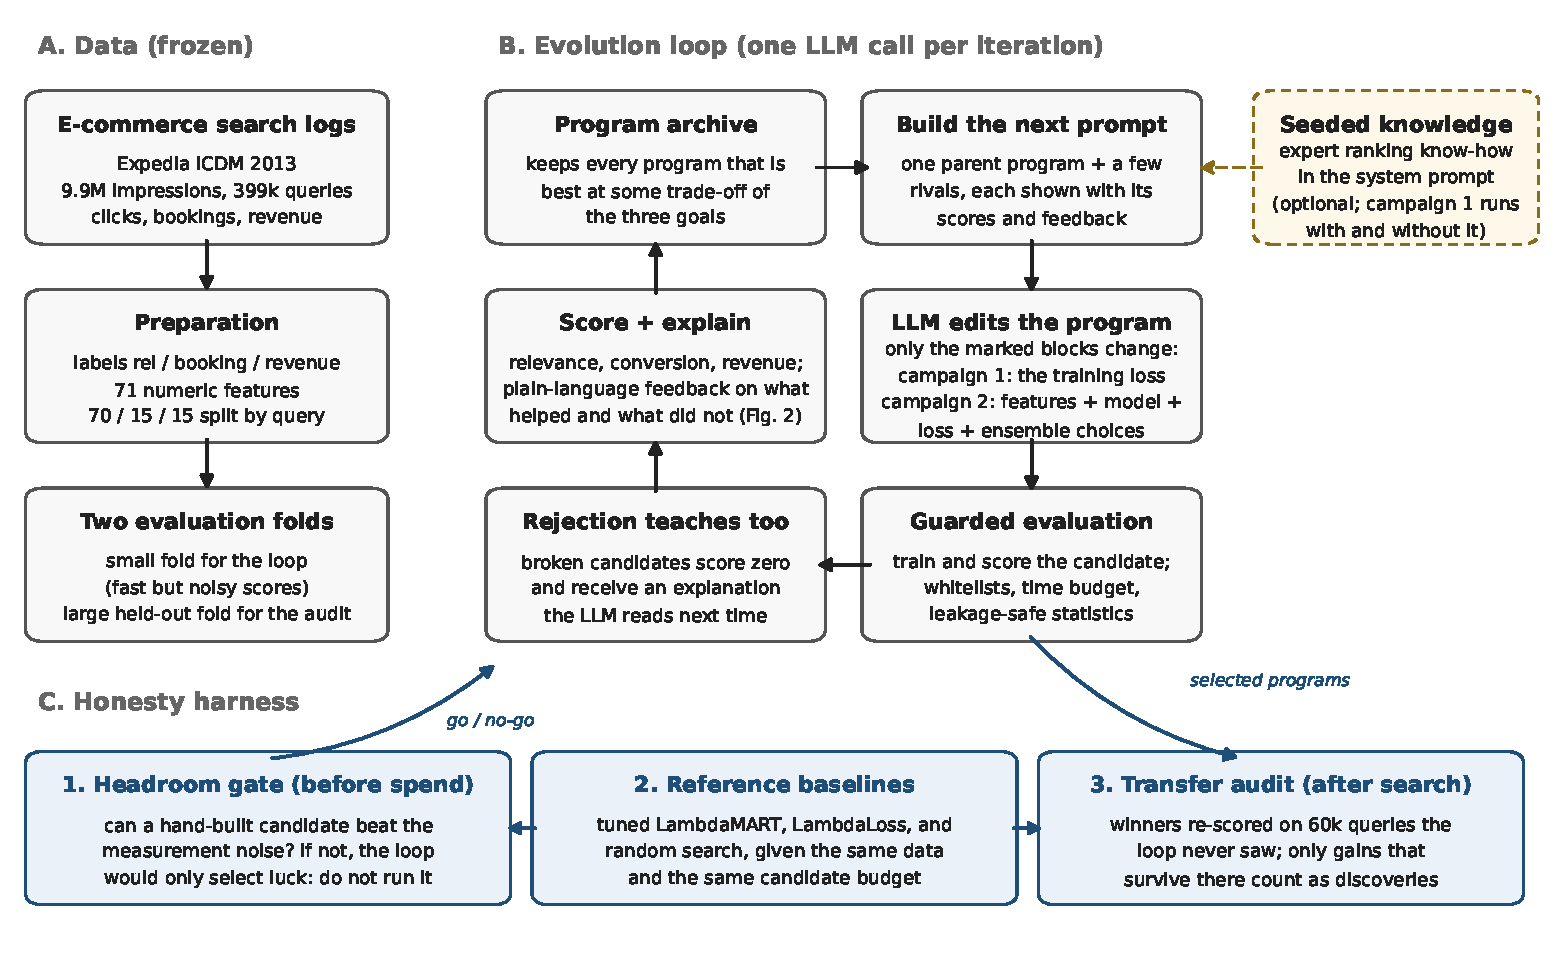
\includegraphics[width=\linewidth]{flowchart.pdf}
  \caption{The EvoRank system. Lane A: data preparation, frozen before any
  search, producing a small fold the loop scores candidates on and a large
  held-out fold it never sees. Lane B: the evolution loop, one LLM call per
  iteration: the archive supplies a parent program and rivals, the LLM edits
  the program's marked blocks, the candidate is trained and scored under
  guardrails, and plain-language feedback (Figure~2) travels back with the
  program into the archive; broken candidates return explanations instead of
  scores. The dashed box is optional expert knowledge in the prompt, ablated
  in campaign 1. Lane C: the honesty harness that brackets the loop: a
  pre-spend gate, baselines on equal terms, and the held-out audit that
  decides what counts as discovered.}
  \label{fig:system}
\end{figure}

\subsection{Background: the evolutionary engine}
EvoRank builds on SkyDiscover, an open framework for LLM-guided evolutionary
program search in the AlphaEvolve family~\cite{alphaevolve,adaevolve};
Figure~\ref{fig:system} shows the assembled system. The unit of evolution is a source
file in which mutable regions are delimited by EVOLVE-BLOCK markers;
everything outside the markers is frozen, which is how we constrain what the
search may change. Each iteration performs one cycle: sample a parent program
(plus a small set of context programs) from a program database, assemble a
prompt containing their source, scores, and evaluator feedback, make a single
LLM call that proposes an edit to the mutable regions, evaluate the resulting
candidate with a user-supplied \texttt{evaluate(program\_path)} function that
returns a metric dictionary, and insert the scored candidate back into the
database. In classical terms, the LLM replaces hand-designed mutation and crossover
operators, and the prompt context plays the role of the mating pool.

We use SkyDiscover's AdaEvolve search controller~\cite{adaevolve}. Its program database is an
island model (two islands here, with dynamic spawning of further islands on
stagnation, up to five) with periodic ring migration of top programs,
which maintains diversity by evolving semi-isolated subpopulations; a
bandit allocates iterations to islands by recent improvement, and each
island adapts its exploration intensity accordingly. In
multi-objective mode the database keeps a Pareto archive: a candidate
survives if no other program dominates it on all objectives (here ndcg,
booking ndcg, and a pooled dollar-weighted revenue metric), with a scalar
fitness key used only for tie-breaking and adaptive-state bookkeeping. On
stagnation the controller can trigger a paradigm step that prompts the LLM
for a high-level strategy change rather than a local edit. All state is checkpointed, so runs resume exactly and every
selected program is preserved with its lineage.

\subsection{Preliminaries: the algorithms in brief}
For readers new to Learning-to-Rank, the recurring machinery is as follows.

\emph{Ranking and NDCG@k.} A search query returns a list of items, each with
a relevance label. NDCG@k scores how well a model orders each list: relevant
items placed near the top earn gain discounted by log-position, normalized by
the best achievable ordering, so 1.0 is a perfect ranking. We compute it per
query and average (for revenue we instead pool dollars across queries, so
high-value queries weigh more).

\emph{GBDT and LambdaMART.} Gradient-boosted decision trees
(XGBoost~\cite{xgboost}, LightGBM~\cite{lightgbm}) fit an additive sequence of small trees, each correcting the
previous ones via gradients of a loss. LambdaMART is the ranking instance:
for every within-query pair where item $i$ outranks item $j$ in the labels,
it applies a pairwise logistic gradient scaled by how much swapping the two
would change NDCG, so training pressure concentrates where the metric is
actually at stake. XGBoost's rank:ndcg and LightGBM's lambdarank implement
it; our campaign-1 candidates are hand-written variants of exactly this
gradient function.

\emph{Hyperparameter tuning with Optuna.} A GBDT's quality depends on
learning rate, depth, subsampling, and regularization. Optuna~\cite{optuna}
searches that space with Bayesian trials scored on validation data. Our
baselines get 40 trials, re-run at every training-set size we report,
because optimal configurations change with the amount of data.

\emph{Ensembling by per-query z-scores.} Different model families make
partially independent errors; because their scores live on different scales,
each model's scores are standardized within each query before a weighted
sum. This was the challenge winners' combiner of choice and is what our
discovered pipelines select.

\emph{Out-of-fold target encoding.} Encoding a categorical column by the
average label of its value (a hotel's historical booking rate) leaks labels
into features unless each row is encoded using statistics from other
query-folds only. Section 5 quantifies what goes wrong otherwise.

\emph{The statistics.} A paired query bootstrap resamples queries and
recomputes the metric difference between two systems thousands of times,
giving intervals that treat the query as the unit of noise. Pareto dominance
means at least as good on every objective and better on one; hypervolume
measures how much objective space the non-dominated set covers.

\subsection{Task, data, and evaluators}
Data is the public Expedia Personalized Hotel Search training file (9.9M
impressions, 399k queries), split 70/15/15 by query, with graded labels (5
booked, 1 clicked, 0 otherwise). A fast fitness fold (8k training queries; the loop scores every candidate
here, and that score is the candidate's fitness) keeps evaluation between 5
and 40 seconds; each candidate trains a
gradient-boosted ranker under a fixed budget and is scored on the fold's
validation queries. Degenerate candidates (non-finite gradients, timeouts, malformed
specifications) receive zero fitness with an explanatory message in the
next prompt, so guardrails double as teaching signals.

\subsection{The audit stack}
The audit stack, applied identically to every campaign, is the methodological
core: (a) paired query bootstrap for every comparison, with noise-gated
deltas inside the loop's own feedback; (b) equal-budget random-search
controls; (c) symmetric hyperparameter treatment (post-hoc Optuna tuning of
discovered artifacts at the baseline's budget); (d) a selection-
generalization audit that rescores every checkpoint's selected program on 60k
held-out queries; (e) three-objective hypervolume; and (f) mechanism
ablations of discovered artifacts. Baselines are LambdaMART (the standard
gradient-boosted ranking algorithm, XGBoost rank:ndcg) with 40 trials of
Optuna hyperparameter search, re-tuned separately at every training-set size
we report, plus an equal-budget random search over the same candidate space as
the loop.
%% TODO: consider a small figure here summarizing the audit stack.

\section{Campaign 1: Objective Space, a Measured Negative}
The evolvable artifact is a group-aware LambdaMART gradient with access to
the raw behavioral signals per impression; training configuration, features,
and metrics are frozen, and the seed reproduces XGBoost's built-in rank:ndcg
within noise.

On the fold the loop selects on, evolved objectives beat the default baseline
and improve steadily. The transfer audit reverses the picture: final selected
objectives gain $+0.0004$ to $+0.0014$ NDCG@10 on held-out queries, the best
evolved objective beats its own seed by $+0.0002$ ($p=0.76$), an equal-budget
random search transfers as well or better ($p=0.03$ in its favor), and every
method is significantly below the tuned baseline ($p=0.0002$). The mechanism
is measured: per-edit effect sizes of 0.002 to 0.005 against a
selection-fold noise floor of $\pm 0.008$ to $0.015$. Enlarging the fitness
fold to 6k queries halves the noise and triples mean transferred gain, the
only intervention that moved transfer.

Guidance ablations: seeding the prompt with curated domain knowledge
reaches the random-search-budget level on the selection fold in 1 to 3
iterations versus 7 to 23 without it, and wins three-objective hypervolume
in every seed, with unchanged transfer. A diagnostic
feedback channel (noise-gated deltas, per-segment breakdowns, probes into
the candidate's actual training gradients) changes nothing measurable across
three seeds. One probe byproduct: the best discovered revenue term moves only 0.09
percent of gradient mass while removing it costs 0.009 revenue, so small but
systematic gradient biases compound across boosting rounds.

Mechanism ablation outperformed further search: knockouts attributed the
best objective's behavior and revealed its per-query adaptive blending was
harmful (a constant blend improved all three metrics), at the cost of five
evaluations. Trained on the full dataset the family is a plateau: everything, including
default rank:ndcg, lands within 0.001 NDCG@10 of everything else.

\section{Campaign 2: Pipeline Space, a Measured Positive}
The second campaign evolves two blocks: feature-construction code over
semantically named columns with a leakage-guarded train-fold statistics API,
and a pipeline specification chosen from a whitelist (one to three members
from XGBoost, LightGBM, and sklearn families with rank, pointwise, binary, or
campaign-1 custom losses, combined by per-query z-score weighting or rank
averaging). Feedback is stage-attributed so the loop can tell which axis
earned each change: a features line, per-member validation scores, the
ensemble's margin over its best member, noise-gated metric deltas, and
segment decompositions.

Figure~\ref{fig:feedback} shows this feedback verbatim; attached to each
candidate in the prompt, it is what the search learns from.

\begin{figure}
\footnotesize
\begin{verbatim}
scores: ndcg=0.4357 (+0.0139 vs seed, +/-0.0054, SIGNIFICANT) |
  book_ndcg=0.4604 (+0.0142, SIGNIFICANT) | revenue=0.4309 (+0.0217, SIGNIFICANT)
features: 80 columns (71 raw + 9 engineered: price_usd_qrank,
  prop_starrating_qrank, prop_review_score_qrank, prop_location_score1_qrank,
  prop_location_score2_qrank, prop_log_historical_price_qrank, prop_id_count,
  dest_count), build 0.6s
members: [0] xgb/rank:ndcg: val ndcg 0.4325 (2s)
         [1] lgbm/lambdarank: val ndcg 0.4261 (4s)
         [2] sklearn/ert: val ndcg 0.4171 (28s)
ensemble: zscore_weighted [0.55, 0.33, 0.12] = 0.4357,
  best single 0.4325 (+0.0033)
segments: booked-q ndcg 0.461 (+0.014 vs seed) | click-only 0.379 (+0.013)
\end{verbatim}
\caption{Stage-attributed feedback for one campaign 2 candidate, verbatim
from the run logs. Deltas are noise-gated against the seed pipeline
reference; per-member lines attribute quality to model and loss choices; the
ensemble line reports the margin over the best single member. Rejected
candidates instead receive an explanatory message, for example the sparsity
floor explaining that per-item rate encodings are data-starved.}
\label{fig:feedback}
\end{figure}

A headroom gate precedes any LLM spend: a hand-built candidate from the ICDM
2013 literature must clear 2.5 times the noise floor, and within-query rank
features plus count encodings did ($+0.013$ NDCG@10). The gate surfaced a
three-generation leakage study we report as a practitioner catalog: naive
train-fold target encoding costs $-0.10$ NDCG (the model memorizes its own
labels); leave-one-out encoding is subtly worse at $-0.13$, because
subtracting the row's own label plants a per-row offset perfectly correlated
with that label, which histogram-based trees read as a label detector; and
query-folded out-of-fold encoding is clean. Each generation was caught by the
audit before any search depended on it.

\begin{table}
  \caption{Campaign 2 transfer audit: fast-train protocol, 59{,}902 held-out
  queries. All three seeds beat the tuned baseline; the best seed dominates
  on all three objectives.}
  \label{tab:transfer}
  \begin{tabular}{lcccc}
    \toprule
    Method & Val NDCG@10 & Test NDCG@10 & Test book & Test revenue \\
    \midrule
    Seed pipeline & 0.4218 & 0.4222 & 0.4443 & 0.4105 \\
    LambdaMART + Optuna & 0.4330 & 0.4296 & 0.4527 & 0.4231 \\
    Pipeline s0 & 0.4356 & 0.4316 & 0.4545 & 0.4257 \\
    Pipeline s1 & 0.4359 & 0.4322 & 0.4553 & 0.4215 \\
    Pipeline s2 & 0.4398 & \textbf{0.4352} & \textbf{0.4582} & \textbf{0.4239} \\
    \bottomrule
  \end{tabular}
\end{table}

Three seeds, 50 iterations each, about 150 LLM calls and ten dollars per
seed, converged on the same interpretable core: five
within-query percentile ranks (price, star rating, review score, location
scores), count encodings of property and destination identifiers, a lean 20
to 30 column feature set whose program comments cite the measured bloat
evidence, and a diverse three-member ensemble (XGBoost rank:ndcg, LightGBM
lambdarank, plus an extra-trees or binary member) under per-query z-score
weighting. One provenance distinction matters for the discovery claim: the
seeded priors included the gate's finding that rank and count features carry
headroom, so their presence is partly prompted; the specific constructions,
the model, loss, ensemble, and weight selections, and the unprompted
inventions (per-query price z-normalization, quantile imputation of a
heavy-missing location score) are the search's own, and the transfer-audited
gains are independent of provenance. Table~\ref{tab:transfer} shows the
transfer audit: roughly 70
percent of selection-fold gains survive on 60k held-out queries, and all
three seeds beat the tuned baseline. A paired query bootstrap (10,000
resamples) makes the headline formal: the best seed beats the tuned baseline
by +0.0057 NDCG@10 (95 percent CI [0.0041, 0.0073], one-sided p < 0.0001)
and +0.0056 booking NDCG@10 (p < 0.0001), while the revenue delta is
positive but within noise (+0.0008, CI [-0.0034, 0.0047]); the
config-equalized full-scale comparison shows the same pattern (+0.0075
NDCG@10, CI [0.0060, 0.0091], p < 0.0001). The frontier claim is therefore
precise: significantly better relevance and conversion at matching revenue.

\begin{table}
  \caption{Full-scale comparison (trained on 280k queries, tested on 60k),
  including NDCG@38, the ICDM 2013 challenge metric. The config-equalized
  pipeline is a lower bound (member configuration not re-tuned for the
  pipeline).}
  \label{tab:fullscale}
  \begin{tabular}{lcccc}
    \toprule
    Method & NDCG@10 & NDCG@38 & Book@10 & Revenue@10 \\
    \midrule
    Tuned baseline (fast-regime config) & 0.4349 & 0.4983 & 0.4588 & 0.4300 \\
    Tuned baseline (full-scale config) & 0.4544 & 0.5132 & 0.4805 & 0.4565 \\
    Pipeline s1 (fast-regime config) & 0.4490 & 0.5080 & 0.4738 & 0.4483 \\
    Pipeline s1 (config-equalized) & \textbf{0.4619} & \textbf{0.5185} & \textbf{0.4883} & \textbf{0.4585} \\
    \bottomrule
  \end{tabular}
\end{table}

The full-data regime required its own rigor step and yields a methodology
lesson (Table~\ref{tab:fullscale}): against a baseline tuned in the fast
regime the pipelines win easily, but re-tuning the baseline at full scale
reverses that naive verdict, and only a config-equalized comparison (the
same tuned hyperparameters on both sides) isolates the discovered structure,
which then wins on all four reported numbers. A
decomposition attributes the margin to both discovered components: the
features alone, under the same tuned single model, reach 0.4587 NDCG@10
(+0.0043 over the strict baseline), and the ensemble adds a further +0.0032
to 0.4619.
We also scored both artifacts on the original competition's hidden test set
via Kaggle late submission (one shot each, no leaderboard iteration): the
discovered pipeline reaches 0.5196 private NDCG@38, which would have placed
20th of 340 teams (top 6 percent) in the 2013 challenge, with the tuned
baseline at 0.5140 (30th), so ten leaderboard places are attributable to the
discovered structure. The winning hand-built ensembles remain ahead (0.5398;
the published solution we cite reports 0.5310), and our submission benefits
from hindsight, since the winners' published lessons are part of the seeded
priors.

\section{Discussion}
The two campaigns differ in exactly one variable, the search space, and the
same loop produced noise in one and transfer-audited Pareto dominance in the
other. The deciding quantity is measurable in advance: the ratio of
achievable effect sizes to fitness-fold noise. We suggest a headroom gate as
cheap preregistration for discovery loops, and transfer-audited selection as
the reporting standard. The positive result is also not specific to the
search algorithm: a threshold-recalibrated AdaEvolve and an EvoX
meta-evolution variant~\cite{evox}, each run at double budget, land within
the original campaign's seed spread on the held-out fold, consistent with
headroom and evaluation fidelity, not search sophistication, governing
outcomes. Guidance (prompt knowledge, evidence-rich feedback)
is a speed and interpretability lever, but in our measurements evaluator-side
investment (larger fitness folds, leakage-safe statistics, stage-attributed
rejection messages the model learns from) carried more of the outcome. The economics compound this: a campaign costs about ten dollars and two
unattended hours, so the relevant unit is gain per human hour; the
hand-built solutions our loop reconstructs took a seven-person team a
competition season.

Limitations: one dataset (newer public datasets lack conversion and
revenue labels, which is why open multi-objective LTR remains anchored to
this benchmark); three seeds per condition; revenue is a proxy metric; and
discovered pipelines were audited for transfer, not online effects.

\section{Conclusion}
Publishing an audited failure next to an audited success on the same task
is more useful than either alone. The loop is neither magic nor
broken: it is a search procedure whose discoveries are real precisely when
the search space offers effect sizes the fitness signal can resolve. Code,
configs, seeds, per-iteration logs, discovered programs, and audit scripts
are released (repository link withheld for double-blind review).

\begin{thebibliography}{99}
\bibitem{funsearch} B. Romera-Paredes, M. Barekatain, A. Novikov, et al.
Mathematical discoveries from program search with large language models.
Nature 625:468--475, 2024.
\bibitem{alphaevolve} A. Novikov, N. V\~{u}, M. Eisenberger, et al.
AlphaEvolve: A coding agent for scientific and algorithmic discovery.
arXiv:2506.13131, 2025.
\bibitem{rea} Meta Engineering. Ranking Engineer Agent (REA): Autonomous AI
system accelerating Meta's ads ranking innovation. Engineering at Meta blog,
March 2026.
\bibitem{adaevolve} M. Cemri, S. Agrawal, A. Gupta, et al. AdaEvolve:
Adaptive LLM Driven Zeroth-Order Optimization. arXiv:2602.20133, 2026.
\bibitem{evox} S. Liu, S. Agarwal, M. Maheswaran, et al. EvoX:
Meta-Evolution for Automated Discovery. arXiv:2602.23413, 2026.
\bibitem{glo} S. Gonzalez and R. Miikkulainen. Improved training speed,
accuracy, and data utilization through loss function optimization. IEEE
Congress on Evolutionary Computation, 2020.
\bibitem{amlfs} C. Li, X. Yuan, C. Lin, et al. AM-LFS: AutoML for Loss
Function Search. ICCV, 2019.
\bibitem{autolosszero} H. Li, T. Fu, J. Dai, et al. AutoLoss-Zero: Searching
Loss Functions from Scratch for Generic Tasks. CVPR, 2022.
\bibitem{cseautoloss} P. Liu, G. Zhang, B. Wang, et al. Loss Function
Discovery for Object Detection via Convergence-Simulation Driven Search.
ICLR, 2021.
\bibitem{lambdaloss} X. Wang, C. Li, N. Golbandi, M. Bendersky, and
M. Najork. The LambdaLoss Framework for Ranking Metric Optimization. CIKM,
2018.
\bibitem{rankevolve} J. Nian, F. Li, D. H. Park, and Y. Fang. RankEvolve:
Automating the Discovery of Retrieval Algorithms via LLM-Driven Evolution.
arXiv:2602.16932, 2026.
\bibitem{reflexion} N. Shinn, F. Cassano, A. Gopinath, K. Narasimhan, and
S. Yao. Reflexion: Language agents with verbal reinforcement learning.
NeurIPS, 2023.
\bibitem{protegi} R. Pryzant, D. Iter, J. Li, Y. T. Lee, C. Zhu, and
M. Zeng. Automatic Prompt Optimization with ``Gradient Descent'' and Beam
Search. EMNLP, 2023.
\bibitem{opro} C. Yang, X. Wang, Y. Lu, et al. Large Language Models as
Optimizers. ICLR, 2024.
\bibitem{gepa} L. Agrawal, S. Tan, D. Soylu, et al. GEPA: Reflective prompt
evolution can outperform reinforcement learning. arXiv:2507.19457, 2025.
\bibitem{caafe} N. Hollmann, S. M\"{u}ller, and F. Hutter. Large Language
Models for Automated Data Science: Introducing CAAFE for Context-Aware
Automated Feature Engineering. NeurIPS, 2023.
\bibitem{aide} Z. Jiang, D. Schmidt, D. Srikanth, et al. AIDE: AI-Driven
Exploration in the Space of Code. arXiv:2502.13138, 2025.
\bibitem{mlagent} Z. Liu, J. Chai, X. Zhu, et al. ML-Agent: Reinforcing LLM
Agents for Autonomous Machine Learning Engineering. arXiv:2505.23723, 2025.
\bibitem{qin2021} Z. Qin, L. Yan, H. Zhuang, et al. Are Neural Rankers
Still Outperformed by Gradient Boosted Decision Trees? ICLR, 2021.
\bibitem{lambdamart} C. J. C. Burges. From RankNet to LambdaRank to
LambdaMART: An overview. Microsoft Research Technical Report MSR-TR-2010-82,
2010.
\bibitem{liu2013} X. Liu, B. Xu, Y. Zhang, et al. Combination of Diverse
Ranking Models for Personalized Expedia Hotel Searches. arXiv:1311.7679,
2013.
\bibitem{survey2024} M. A. Kabir, M. A. Hasan, A. Mandal, D. Tunkelang, and
Z. Wu. A Survey on E-Commerce Learning to Rank. arXiv:2412.03581, 2024.
\bibitem{optuna} T. Akiba, S. Sano, T. Yanase, T. Ohta, and M. Koyama.
Optuna: A Next-generation Hyperparameter Optimization Framework. KDD, 2019.
\bibitem{xgboost} T. Chen and C. Guestrin. XGBoost: A Scalable Tree Boosting
System. KDD, 2016.
\bibitem{lightgbm} G. Ke, Q. Meng, T. Finley, et al. LightGBM: A Highly
Efficient Gradient Boosting Decision Tree. NeurIPS, 2017.
\end{thebibliography}

\end{document}
